\chapter{Literature Review}\label{ch:lit}

\section{Thermoelectric Materials and Device Trends}
Classical Bi$_2$Te$_3$-based systems remain dominant near room temperature, while skutterudites, half-Heuslers, and SnSe address higher-temperature windows \citep{rowe1995crc,disalvo1999thermoelectric,pei2012convergence}. Nanostructuring has delivered major gains by reducing lattice thermal conductivity through intensified phonon scattering \citep{venkatasubramanian2001thin,hochbaum2008enhanced,biswas2012high}.

\section{PCM-Assisted Thermal Management}
PCMs can buffer thermal shocks and maintain near-isothermal boundaries around their melting interval. Reviews report paraffin, salt hydrates, and fatty-acid families for electronics and energy devices \citep{khan2017reviewpcm,sharma2009review}. In thermoelectric contexts, PCM coupling is less mature and often lacks formal exergy accounting under cyclical operation \citep{li2019tepcm}.

\section{Polymer Scaffolds for PCM Confinement}
Porous polymers, aerogels, and cryogels are attractive as leakage-resistant hosts \citep{song2018shape}. PVA is notable due to hydrophilicity, processability, hydrogen bonding, and tunable crystallinity \citep{chiellini2003pva}. Yet few studies combine hierarchical porosity, conductive nanofillers, and thermoelectric mission profiles.

\section{Nanofiller Reinforcement in PVA Composites}
Transition-metal sulfides and 2D dichalcogenides can increase carrier pathways and interfacial polarization effects in polymers \citep{wang2018mos2,liang2021cus}. Hybrid CuS--MoS$_2$ heterostructures are especially promising for synergistic conduction networks and interfacial phonon control \citep{zhou2022hetero}.

\begin{equation}\label{eq:lit_eff_gap}
\eta_{TE}=\frac{\Delta T}{T_h}\frac{\sqrt{1+ZT_{avg}}-1}{\sqrt{1+ZT_{avg}}+T_c/T_h}
\end{equation}
shows why transiently preserving $\Delta T$ can materially influence conversion efficiency.

\begin{equation}\label{eq:lit_cycle_metric}
\Gamma=\frac{1}{N}\sum_{n=1}^{N}\left|\Delta T_n-\overline{\Delta T}\right|
\end{equation}
can be used as a cycle-stability indicator minimized through PCM buffering.

\begin{figure}[htbp]
\centering
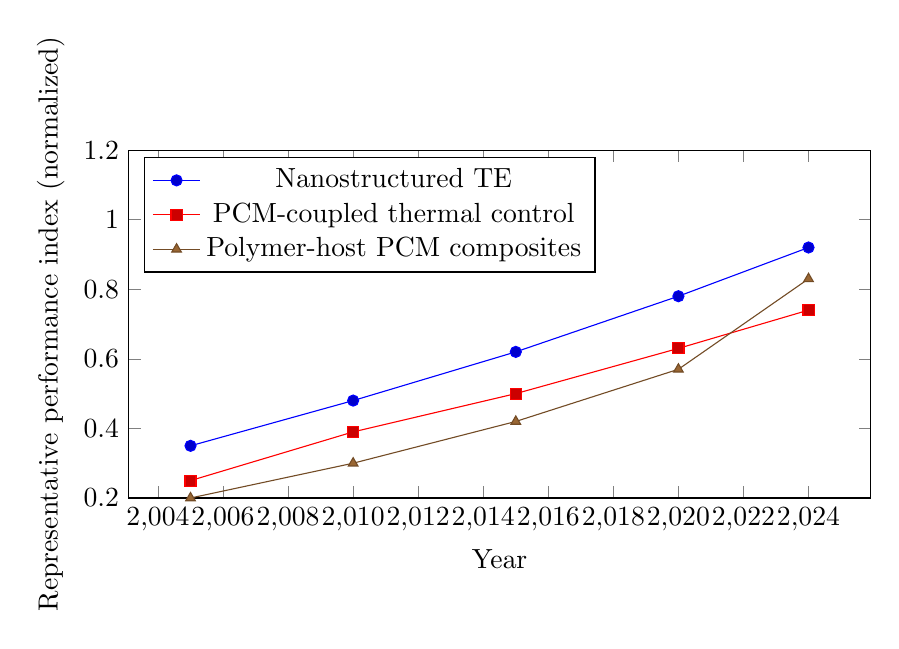
\begin{tikzpicture}
\begin{axis}[
width=11cm,height=6cm,
xlabel={Year},ylabel={Representative performance index (normalized)},
legend style={at={(0.02,0.98)},anchor=north west},
ymin=0.2,ymax=1.2]
\addplot+[mark=*] coordinates {(2005,0.35)(2010,0.48)(2015,0.62)(2020,0.78)(2024,0.92)};
\addlegendentry{Nanostructured TE}
\addplot+[mark=square*] coordinates {(2005,0.25)(2010,0.39)(2015,0.50)(2020,0.63)(2024,0.74)};
\addlegendentry{PCM-coupled thermal control}
\addplot+[mark=triangle*] coordinates {(2005,0.20)(2010,0.30)(2015,0.42)(2020,0.57)(2024,0.83)};
\addlegendentry{Polymer-host PCM composites}
\end{axis}
\end{tikzpicture}
\caption{Indicative evolution of related research streams motivating integrated TE--PCM--PVA design.}
\label{fig:lit_trends}
\end{figure}

\begin{table}[htbp]
\centering
\caption{Literature gap synthesis relevant to this dissertation.}
\label{tab:lit_gap}
\begin{tabular}{p{4cm}p{3.5cm}p{4.2cm}}
\toprule
Theme & Typical prior focus & Remaining gap \\
\midrule
TE optimization & Static $ZT$ maximization & Limited transient buffering analysis \\
PCM integration & Bulk thermal storage & Weak coupling to TE transport equations \\
Polymer hosts & Shape stability only & Insufficient multiphysics role separation \\
Nanofillers in polymers & Conductivity increase & Sparse exergy/entropy interpretation \\
\bottomrule
\end{tabular}
\end{table}
